\subsection{Stream Partitioning}
We use the Geohash~algorithm~\cite{geohash} to balance load and partition incoming data streams across processing resources. Geohash divides the earth into a hierarchy of bounding boxes identified by Base 32 strings; the longer the Geohash string, the more precise the bounding box. Figure~\ref{fig:geohash} illustrates this hierarchy; most of the western United States and Mexico are contained within the bounding box described by Geohash string \emph{9}, while \emph{9Q} encompasses parts of California, Nevada, Arizona, and Utah. The bounding box \emph{9Q9K} (highlighted in red) contains San Jose, California. This hierarchical representation enables \textsc{Rivulet} to cope with both low- and high-density regions. For instance, several resources may be tasked with managing streams originating in and around the San Francisco region, while the entirety of Yosemite National Park could fall under the purview of a single node.

\begin{figure}
    \centerline{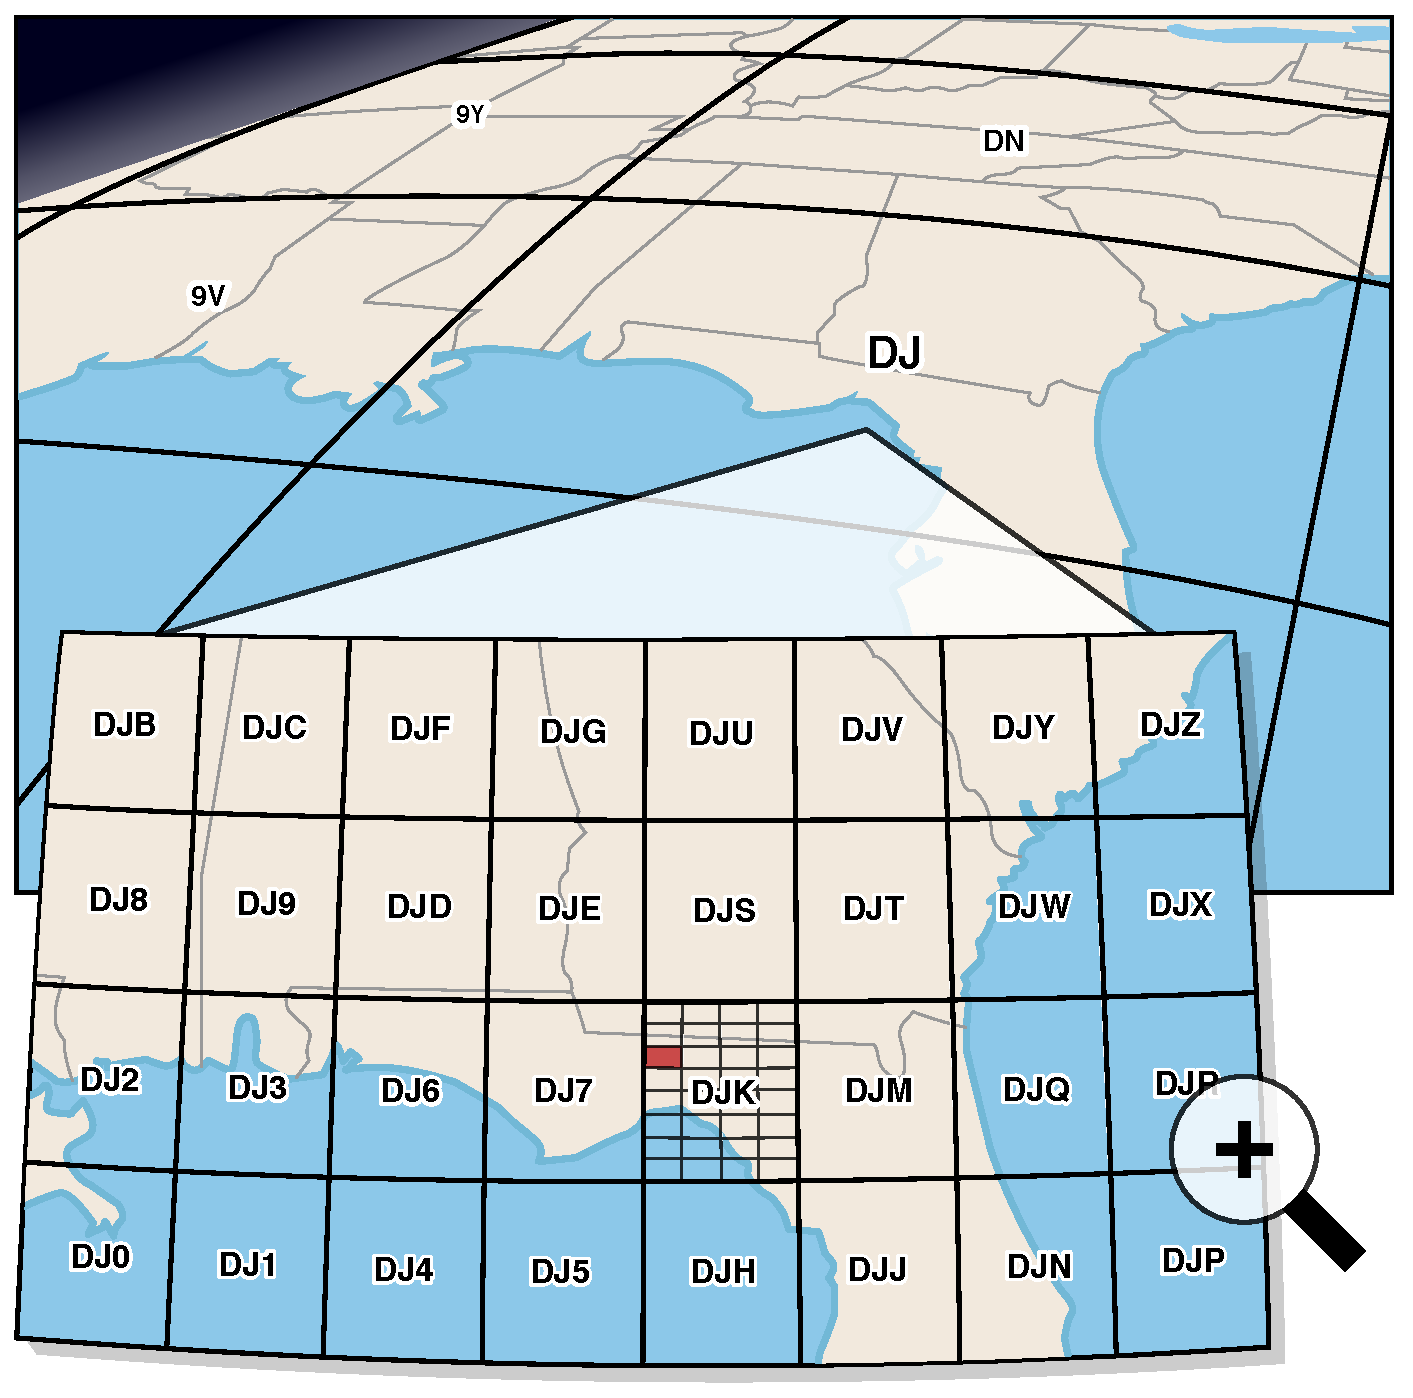
\includegraphics[width=3.5in]{figures/geohash.pdf}}
    \caption{A demonstration of the Geohash algorithm. Each additional character in a Geohash string describes a finer-grained region; Geohash \emph{9Q} contains a substantial portion of California, USA, while \emph{9Q9K} (highlighted in red) represents a smaller region containing San Jose, California.}
    \label{fig:geohash}
\end{figure}

To achieve fine-grained control over our Geohash partitions, we operate at the bit level rather than Base 32 character level when routing streams. Each bit added to a Geohash string reduces its scope by half, with each character represented by five bits ($2^5 = 32$). In other words, a four-character Geohash string represents 20 spatial subdivisions. This property allows us to manage and allocate resources across a wide variety of observational densities.

